\documentclass{beamer}
\usetheme{Dresden}
\usepackage{graphicx}
\usepackage{pifont}
\usepackage[activate={true,nocompatibility},final,tracking=true,kerning=true,spacing=true,factor=1100,stretch=10,shrink=10,expansion]{microtype}
\usepackage[utf8]{inputenc}              %%Formatação de acentos
\usepackage{xcolor}                      %%Definição de cores
\usepackage[framemethod=tikz]{mdframed} %%Estilização dos slides
\usepackage{tcolorbox}                   %%Mudar ambientes de blocos
\usepackage[alf]{abntex2cite}

\title[Alumínio]{Produção de Alumínio}
\author[Valentina Santana]{Valentina Santana Santos \\
  Valssantos@usp.br}
\date[2020]{2020}

\begin{document}

\begin{frame}
  \maketitle
\end{frame}


\begin{frame}
  \frametitle{Etapas da Produção}

  \begin{itemize}
  \item[\color{red}]Extração
  \item[\color{red}]Refino - Processo Bayer \cite{martires2009}
  \item[\color{red}]Redução - Processo Hall-Héroult \cite{massara2004}
  \item[\color{red}]Aplicação do Alumínio Primário
  \end{itemize}

\end{frame}

\begin{frame}
  \frametitle{Visão Geral do Processo}

  \begin{tcolorbox}

  \begin{figure}
    \caption{Fluxograma Produção de Alumínio Primário}
    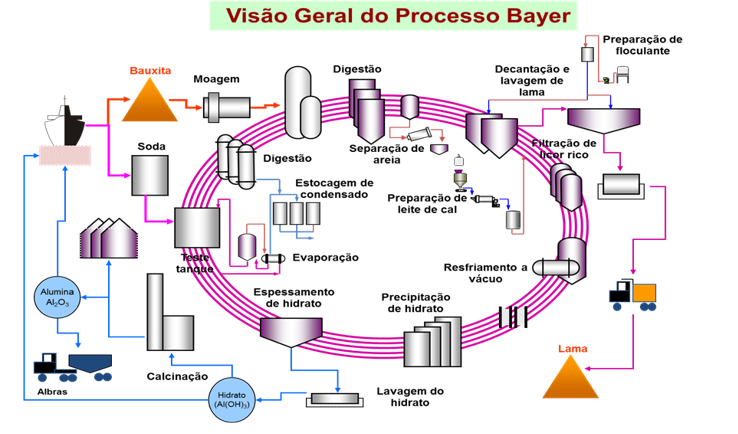
\includegraphics[width=0.4\linewidth]{aluminio_bayer.png}

    \legend{Comentários/Fonte \footnote{algum comentário técnico}}
  \end{figure}
\end{tcolorbox}

\end{frame}


\begin{frame}
  \frametitle{Referências}
  \bibliography{ref}
\end{frame}

\end{document}

%%% Local Variables:
%%% mode: latex
%%% TeX-master: t
%%% End:
